\section{Linear Programming}
\subsection{What's Linear Programming ?}
\begin{tcolorbox}[title = Definition] 
    tcolorbox
\end{tcolorbox}
\vspace{1cm}
\begin{center}
    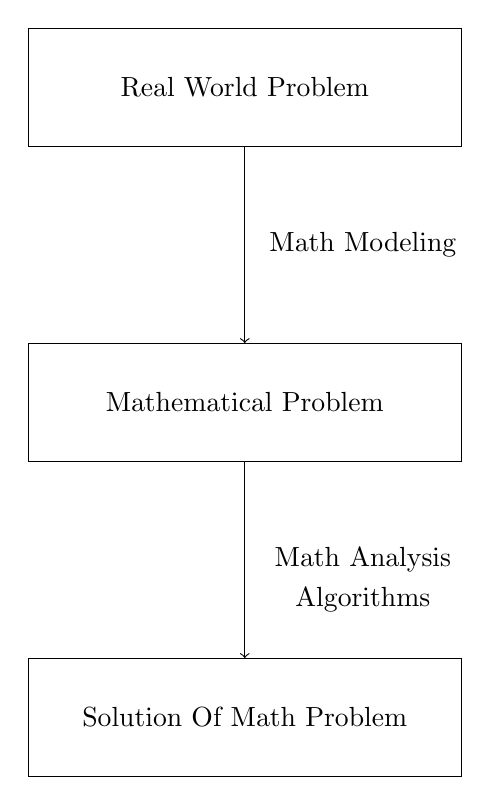
\begin{tikzpicture}
       \draw (0,0) rectangle (5.5,1.5);
       \node at (2.75,0.75) {Real World Problem};
      
       \draw[->] (2.75,0) -- (2.75,-2.5);
       \node at (4.25,-1.25) {Math Modeling};

       \draw (0,-4) rectangle (5.5,-2.5);
       \node at (2.75,-3.25) {Mathematical Problem};
      
       \draw[->] (2.75,-4) -- (2.75,-6.5);
       \node at (4.25,-5.25) {Math Analysis};
       \node at (4.25,-5.75) {Algorithms};
       
       \draw (0,-8) rectangle (5.5,-6.5);
       \node at (2.75,-7.25) {Solution Of Math Problem};
   \end{tikzpicture}
\end{center}
\vspace{1cm}
\subsection{Modeling}
\textbf{\large{\underline{Example :} Diet Problem}}\\

\vspace{0.25cm}
The Goal is to minimize food cost but to meet the minimum daily nutrition requirement
\vspace{1cm}
\begin{center}
\begin{tabular}{|c|c|c|c|c|c|}
    \hline
    Food & Units & Protein & Vit c & Iron & Price\\
    \hline
    Apples & 1 med & 0.4 & 6 & 0.4 & 8\\
    \hline
    Banana & 1 med & 1.2 & 10 & 0.6 & 10\\
    \hline
\end{tabular}
\end{center}

\vspace{1cm}

\begin{multicols}{2}
\textbf{\underline{Variables Definition:}}\\

Let \(x_1\) be the number of Daily Unit Appels.\\

Let \(x_2\) be the number of Daily Unit Banana.\\
\columnbreak

\textbf{\underline{Constraint:}} 

\[
\left\{
    \begin{array}{l}
        \forall x_1 , x_2 \geq 0 \quad \text{(Non-negative number of food item) ...C1}\\\\
        0.4x_1 + 1.2x_2  \geq 70 \quad \text{(Minimum Protein Daily) ...C2}\\\\ 
        6x_1 + 10x_2  \geq 50 \quad \text{(Minimum Vitamine c Daily) ...C3}\\\\
        0.4x_1 + 0.6x_2  \geq 12 \quad \text{(Minimum Iron Daily) ...C4}
   \end{array}
   \right.
\] 
\end{multicols}
\vspace{0.5cm}
\begin{tcolorbox}[title = Objectif Function]
\[
f(x) = 8x_1 + 10x_2  
\]
\begin{center}
The goal is to minimize food cost by maximizing \(f(x)\), while meeting the minimum daily nutrition .
\end{center}
\end{tcolorbox}
\vspace{1cm} 
\textbf{\underline{Problem :}} Find the minimum of \(f(x_1,x_2) \) subject to the contraints\\
\subsection{Graph Model}
This model is used when the objective fucntion has 2 variables consist into turning all the constraint into 
lines and then finding the feasible region and then to search for min or max of the objective function 

\vspace{1cm}
\textbf{Feasible Region :}

\vspace{1cm}
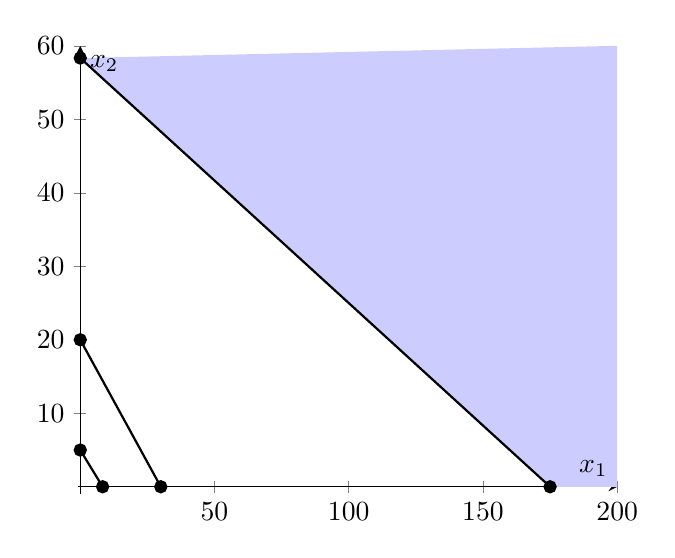
\begin{tikzpicture}
    \begin{axis}[
        axis lines = middle,           % Ensures axes cross at (0, 0)
        xlabel=$x_1$, 
        ylabel=$x_2$, 
        xmin = -1, xmax = 200,           % Set x-axis range
        ymin = -1, ymax = 60,           % Set y-axis range
       ytick={0,10,...,70},             % Y-tick values
        xtick={0,50,...,200},
    ]
  \addplot [draw=none, fill=blue!20] coordinates {(175,0) (200,0) (200,60) (0,70/1.2)}; 
  \addplot[thick, mark=*] coordinates {(175,0) (0,70/1.2)}; 
  \addplot[thick, mark=*] coordinates {(50/6,0) (0,5)};
  \addplot[thick, mark=*] coordinates {(30,0) (0,20)};
\end{axis}

\end{tikzpicture}
